% $Id: template.tex 11 2007-04-03 22:25:53Z jpeltier $

%\documentclass{vgtc}                          % final (conference style)
%\documentclass[review]{vgtc}                 % review
%\documentclass[widereview]{vgtc}             % wide-spaced review
\documentclass[preprint]{vgtc}               % preprint
%\documentclass[electronic]{vgtc}             % electronic version

%% Uncomment one of the lines above depending on where your paper is
%% in the conference process. ``review'' and ``widereview'' are for review
%% submission, ``preprint'' is for pre-publication, and the final version
%% doesn't use a specific qualifier. Further, ``electronic'' includes
%% hyperreferences for more convenient online viewing.

%% Please use one of the ``review'' options in combination with the
%% assigned online id (see below) ONLY if your paper uses a double blind
%% review process. Some conferences, like IEEE Vis and InfoVis, have NOT
%% in the past.

%% Figures should be in CMYK or Grey scale format, otherwise, colour 
%% shifting may occur during the printing process.

%% These few lines make a distinction between latex and pdflatex calls and they
%% bring in essential packages for graphics and font handling.
%% Note that due to the \DeclareGraphicsExtensions{} call it is no longer necessary
%% to provide the the path and extension of a graphics file:
%% \includegraphics{diamondrule} is completely sufficient.
%%
\ifpdf%                                % if we use pdflatex
  \pdfoutput=1\relax                   % create PDFs from pdfLaTeX
  \pdfcompresslevel=9                  % PDF Compression
  \pdfoptionpdfminorversion=7          % create PDF 1.7
  \ExecuteOptions{pdftex}
  \usepackage{graphicx}                % allow us to embed graphics files
  \DeclareGraphicsExtensions{.pdf,.png,.jpg,.jpeg} % for pdflatex we expect .pdf, .png, or .jpg files
\else%                                 % else we use pure latex
  \ExecuteOptions{dvips}
  \usepackage{graphicx}                % allow us to embed graphics files
  \DeclareGraphicsExtensions{.eps}     % for pure latex we expect eps files
\fi%

%% it is recomended to use ``\autoref{sec:bla}'' instead of ``Fig.~\ref{sec:bla}''
\graphicspath{{figures/}{pictures/}{images/}{./}} % where to search for the images

\usepackage{svg}

\usepackage{microtype}                 % use micro-typography (slightly more compact, better to read)
\PassOptionsToPackage{warn}{textcomp}  % to address font issues with \textrightarrow
\usepackage{textcomp}                  % use better special symbols
\usepackage{mathptmx}                  % use matching math font
\usepackage{times}                     % we use Times as the main font
\renewcommand*\ttdefault{txtt}         % a nicer typewriter font
\usepackage{cite}                      % needed to automatically sort the references
\usepackage{tabu}                      % only used for the table example
\usepackage{booktabs}                  % only used for the table example
%% We encourage the use of mathptmx for consistent usage of times font
%% throughout the proceedings. However, if you encounter conflicts
%% with other math-related packages, you may want to disable it.


%% If you are submitting a paper to a conference for review with a double
%% blind reviewing process, please replace the value ``0'' below with your
%% OnlineID. Otherwise, you may safely leave it at ``0''.
\onlineid{0}

%% declare the category of your paper, only shown in review mode
\vgtccategory{Research}

%% allow for this line if you want the electronic option to work properly
\vgtcinsertpkg

%% In preprint mode you may define your own headline. If not, the default IEEE copyright message will appear in preprint mode.
%\preprinttext{To appear in an IEEE VGTC sponsored conference.}

%% This adds a link to the version of the paper on IEEEXplore
%% Uncomment this line when you produce a preprint version of the article 
%% after the article receives a DOI for the paper from IEEE
%\ieeedoi{xx.xxxx/TVCG.201x.xxxxxxx}


%% Paper title.
%% Abstract section.
\abstract{Screen-based Augmented Reality (AR), such as on handheld devices, is a convenient and accessible way to enrich our environment with virtual imagery. Common limitations of such a display are that it presents a monocular view of the environment where the image plane is located on the display. Since the display is closer to the viewer, either it or the environment is not in focus. Stereoscopic displays allow each eye to have a different view and thus allow them to converge on a variable depth, however having a different distance for eye vergence and accommodation is known to cause discomfort (vergence-accommodation conflict). These limitations could make it more difficult to merge the AR content on the screen-based display with its surroundings, a significant problem when usage requires rapid shifts between the two (e.g. when validating augmented instructions before making incision, cutting the wire, general hand-eye coordinated tasks such as grasping for augmented objects, etc.). To investigate the relative influence of accommodation and vergence on merging AR content we run two user studies with 9 and 27 participants and found that when rapidly switching gaze between the display and the environment, minimising accommodation difference plays a key role, wheras when viewing the display and the environment as a single merged contex without switching gaze, vergence prevails. Furthermore vergence-accommodation conflict did not impact cognitive workload nor was it detected as an important factor for accurate merging of the AR conten.   
Based on this we propose design recommendations for scenarios that utilize a screen-based AR display.
} % end of abstract

\title{Effects of Eye Vergence and Accommodation on Merging an AR Magic
Lens Display with its Surrounding Real Environment}
\author{Geert Lugtenberg}
\date{November 2023}

\begin{document}

\maketitle

\section{Introduction}
Augmented Reality (AR) has long been envisaged as a support system
for both everyday and specialized tasks [3]. These amongst
others include teaching [1] and learning [2]. Since smartphones
equipped with dedicated graphical processing units, high quality
cameras and displays became readily available, the world augmented
by virtual imagery became easily accessible to the common consumer
with minimum extra effort or costs. By utilizing the smartphone
camera image, a user is able to view the physical world together
with digital content as if the handheld device is a transparent
screen or lens, sometimes called a Magic Lens (ML) display.

\section{BACKGROUND & RELATED WORK}
In order to explore accommodation and vergence influence on merging
a screen with its surroundings we first need to explore how these
eye phenomena affect our regular daily vision.

\subsection{Accommodation and eye strain}
In order to bend light diffusing from a surface so that it ends up in
focus on your retina, the muscles in your eye contract the lens in
your eye, making it more or less convex. When this accommodation
process does not work well enough, usually with older age, objects
near the eye (hyperopia) or in the distance (myopia) become blurry.
Myopia is a common phenomenon occurring in about 10\% of people
\begin{figure}[h] % here top bottom [h][t][b] ("!" overwrite-a)
    \centering
    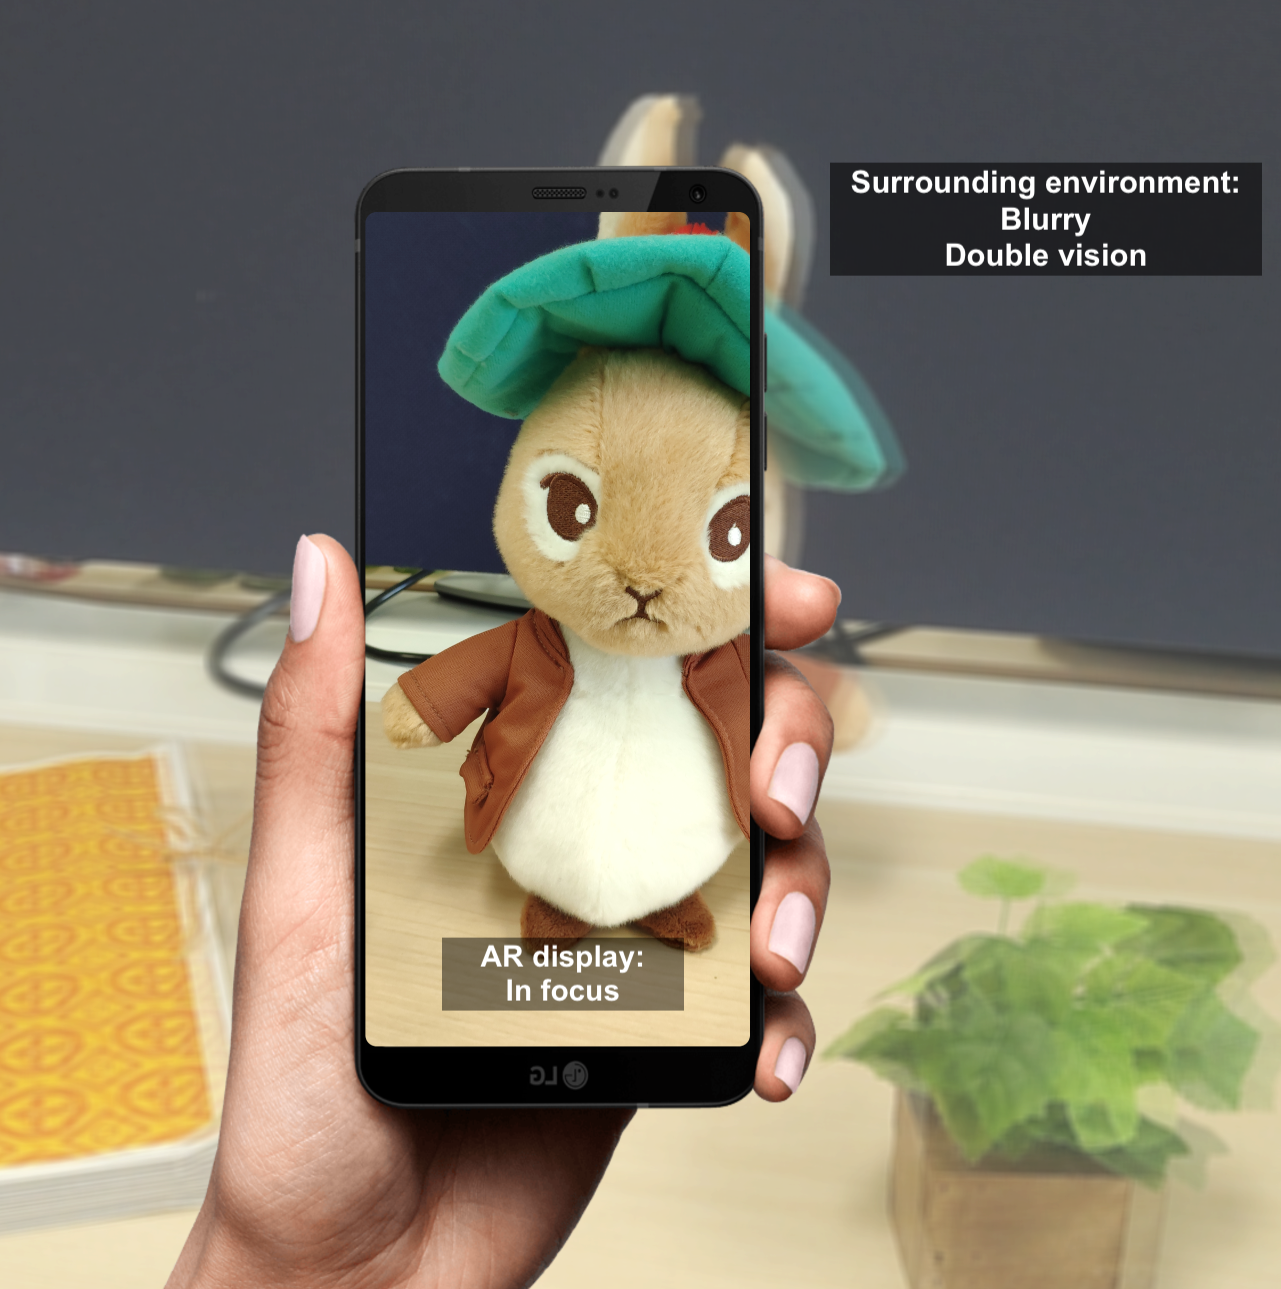
\includegraphics[width=\linewidth]{RP1_preverjanje znanja/figures/Focus and diplopia on ML display.png}
    \caption{Display content as rendered from the perspective of the
user. Focusing on the handheld display causes the surrounding
environment to become blurred and double (diplopia) due to eye
accommodation and vergence respectively.}
    \label{fig:nemo}
\end{figure}
, varying with age, ethnicity and lifestyle. Both conditions can be
corrected with convex or concave lenses in spectacles or contact
lenses, but left untreated cause eye fatigue and headaches in addition
to impairment of activities. Some studies suggest that prolonged
use of near-view displays such as computer monitors, tablets and
smartphones also cause accommodation-related symptoms and subsequently
eye discomfort. In mixed reality systems, due to virtual
content always being displayed at fixed focal distance, the logical
result is that there is often a discrepancy in accommodation distance
between the virtual and the real, causing either to be out of focus. Related
work in augmented reality systems using head-worn displays
investigate ways to relieve this issue; through vari-focal technology
where the focal point is mechanically changed or multiple focal
planes exist. Near-eye light field displays tackle the accommodation
issue by rendering the scene from many view angles resulting in
different depths per view angle. There are techniques such as the
Maxwellian view that project the virtual image onto a specific part of
the eye retina, most commonly the fovea. This requires careful calibration
taking into account the positional relationship between the
eyes and display, and has been used in HWDs before. Interestingly,
screen-based augmented reality, such as those using handheld devices
or Magic Lenses, have the same accommodation issues (since
the virtual content focal plane is fixed at arm’s length) but is far
less investigated than their HWD counterpart, partly motivating the
proposed work here.
\newpage


\begin{table}[h]

    \caption{Subjective grading of performance per condition and display
type for User study B}
    \label{tab:seznam}
    \centering
    \begin{tabular}{c|c c|c c c c | c}
        \hline
         Transparent & FAR & FAR & 20 & 2 & 3 & 1 & 93 \\
         Transparent & FAR & FAR & 20 & 2 & 3 & 1 & 93 \\
         Transparent & FAR & FAR & 20 & 2 & 3 & 1 & 93 \\
         Transparent & FAR & FAR & 20 & 2 & 3 & 1 & 93 \\
         \hline
    \end{tabular}
\end{table}

\cite{6402557}
\cite{7893336}
\cite{bababekova2011font}

\bibliographystyle{abbrv-doi}
\bibliography{template}
\end{document}
